\documentclass[a4paper,12pt,titlepage]{article}
\usepackage{luatexja}

\usepackage{graphicx}
\usepackage{amsmath}
\usepackage[colorlinks=true,linkcolor=blue,urlcolor=blue,citecolor=blue]{hyperref}
\usepackage{geometry}
\geometry{margin=25mm}
\setlength{\parindent}{0pt}
\setlength{\parskip}{1em}

\usepackage{listings}
\lstset{
  basicstyle={\ttfamily},
  identifierstyle={\small},
  commentstyle={\smallitshape},
  keywordstyle={\small\bfseries},
  ndkeywordstyle={\small},
  stringstyle={\small\ttfamily},
  frame={tb},
  breaklines=true,
  columns=[l]{fullflexible},
  numbers=left,
}

\begin{document}

%--------------------------------------------------------------------------------------------------
% Title
%--------------------------------------------------------------------------------------------------

\title{MODELngspicer User Guide}
\author{ペE}
\date{\today}
\maketitle

\tableofcontents
\newpage

%--------------------------------------------------------------------------------------------------
% Section: Introduction
%--------------------------------------------------------------------------------------------------
\section{Introduction}

\textbf{MODELngspicer} is a GUI application built on top of ngspice, designed to help circuit
design optimization and device modeling. The graphical interface is developed using Qt library
(PySide6), allowing users to adjust circuit parameters intuitively and visualize simulation results
in real time. This seamless integration between control and feedback enables rapid iteration and
deeper insight into circuit behavior.

\textbf{Ngspice} (\url{https://ngspice.sourceforge.io}) is an open-source SPICE circuit simulator
that supports a wide range of analyses, including DC, AC, transient, noise, distortion, and
S-parameter analysis. It also accommodates industry-standard models such as Verilog-A and BSIM,
enabling high-precision device modeling. Since it operates via command line, ngspice is well suited
for complex scripted computations and automated analysis workflows.

%--------------------------------------------------------------------------------------------------
% Section: Installation
%--------------------------------------------------------------------------------------------------
\section{Installation}

%--------------------------------------------------------------------------------------------------
% Subsection: System Requirements
%--------------------------------------------------------------------------------------------------
\subsection{System Requirements}

MODELngspicer has been tested under the following environment:

\begin{itemize}
    \setlength{\parskip}{0mm}
    \setlength{\itemsep}{0mm}
    \item Operating system: Windows 10 or later (64-bit)
    \item Python: Version 3.13 or later
    \item Required packages: PySide6, PyQtGraph, NumPy
    \item Ngspice: Version 41 or later
\end{itemize}

%--------------------------------------------------------------------------------------------------
% Subsection: Installation on Windows
%--------------------------------------------------------------------------------------------------
\subsection{Installation on Windows}

This section outlines the installation procedure using Chocolatey, a package manager for Windows.

\begin{enumerate}
    \item Install Chocolatey\\
        Open PowerShell as Administrator and run the following command.
        For more details, visit Chocolatey's official installation page
        (\url{https://chocolatey.org/install}).

\begin{verbatim}
Set-ExecutionPolicy Bypass -Scope Process -Force; `
[System.Net.ServicePointManager]::SecurityProtocol = `
[System.Net.ServicePointManager]::SecurityProtocol -bor 3072; `
iex ((New-Object System.Net.WebClient).DownloadString(`
'https://community.chocolatey.org/install.ps1'))
\end{verbatim}

    \item Install Python and Ngspice\\
        Run the following commands in an administrator PowerShell to install Python and Ngspice.
        After installation, verify that \texttt{python}, \texttt{pip}, and \texttt{ngspice\_con}
        commands are available.

\begin{verbatim}
choco install python
choco install ngspice
\end{verbatim}

    \item Install required packages\\
        Run the following command to install required Python libraries.

\begin{verbatim}
pip install pyside6 pyqtgraph numpy
\end{verbatim}

    \item Launch the application\\
        Once the setup is complete, you can launch MODELngspicer by double-clicking
        \texttt{run.vbs} or \texttt{run.bat} located in the project folder.

\end{enumerate}

%--------------------------------------------------------------------------------------------------
% Section: GUI and Basic Operations
%--------------------------------------------------------------------------------------------------
\section{GUI and Basic Operations}

%--------------------------------------------------------------------------------------------------
% Subsection: Interface Overview
%--------------------------------------------------------------------------------------------------
\subsection{Interface Overview}

Figure \ref{fig:img01} shows the graphical interface layout.

\begin{figure}[htbp]
    \centering
    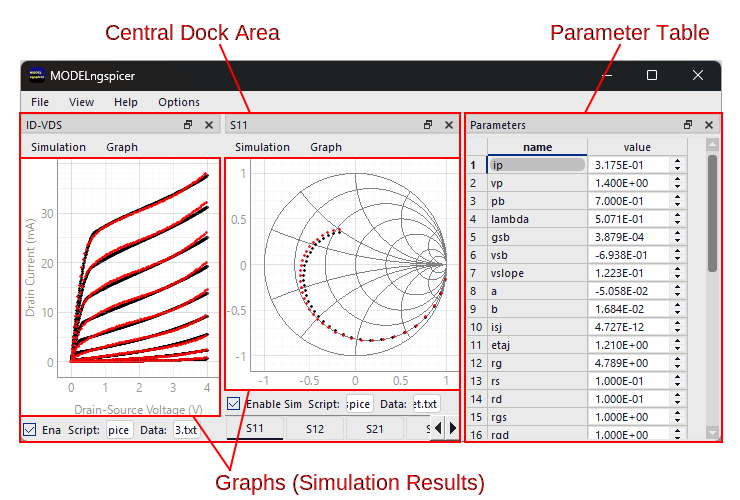
\includegraphics[width=0.8\textwidth]{images/img01.pdf}
    \caption{Graphical interface}
    \label{fig:img01}
\end{figure}

\begin{itemize}
    \setlength{\parskip}{0mm}
    \setlength{\itemsep}{0mm}
    \item \textbf{Central Dock Area}\\
        The area where the simulation widgets are stored. Up to 10 pages can be added.
    \item \textbf{Parameter Table}\\
        Displays a list of parameters loaded from "File > Import Params...".
        Each parameter value is shown in a spin box and can be adjusted using a mouse wheel.
    \item \textbf{Graph}\\
        Simulation results and measurement data are plotted. Simulation results are shown as black
        dots, while measurement data as red dots.
\end{itemize}

%--------------------------------------------------------------------------------------------------
% Subsection: Operation Flow
%--------------------------------------------------------------------------------------------------
\subsection{Operation Flow}

The user needs to prepare at least the following two files. The formats of these files are
explained in the next section.

\begin{itemize}
    \setlength{\parskip}{0mm}
    \setlength{\itemsep}{0mm}
    \item Parameter definition file
    \item Ngspice script file
\end{itemize}

The basic operation workflow is outlined below.

\begin{enumerate}
    \item \textbf{Import parameters}\\
        Select a parameter definition file via "File > Import Params...".
        The loaded parameters will be displayed in the parameter table.
    \item \textbf{Select ngspice script}\\
        Select an ngspice script (.spice, .sp, or .cir) via
        "Simulation > Select Ngspice Script...".
    \item \textbf{Select external data (optional)}\\
        Load external data such as measurement results or target values via
        "Simulation > Select Data...".
    \item \textbf{Enable/Disable simulation (optional)}\\
        Simulation can be toggled via "Simulation > Enable/Disable Simulation" or the check box at
        the bottom left of the simulation widget. Disabling unused simulations may help reduce
        execution time.
    \item \textbf{Adjust parameters}\\
        Adjust parameter values using the spin boxes in the parameter table.\\
        - Mouse wheel \rightarrow\ fine adjustment\\
        - Ctrl + mouse wheel \rightarrow\ coarse adjustment
    \item \textbf{Review results}\\
        Simulation results and external data are plotted in the graph.
    \item \textbf{Save parameters}\\
        Save the adjusted parameters via "File > Export Params..."
\end{enumerate}

%--------------------------------------------------------------------------------------------------
% Section: File Formats
%--------------------------------------------------------------------------------------------------
\section{File Formats}

%--------------------------------------------------------------------------------------------------
% Subsection: Parameter Definition File
%--------------------------------------------------------------------------------------------------
\subsection{Parameter Definition File}

Parameters are defined in a plain text (.txt). Each line must begin with a "+" symbol as shown in
Listing \ref{listing01}. The "+" symbol is part of SPICE syntax and indicates a continuation from
the previous line. By using this format, the parameter definitions can be seamlessly expanded into
\texttt{.param} or \texttt{.model} statements within SPICE scripts.

\begin{lstlisting}[label=listing01,caption=Example of parameter definition]
+ is = 1e-14
+ n = 1.5
+ rs = 0.5
+ ...
\end{lstlisting}

Listing \ref{listing02} shows an example of an SPICE script expanding the parameter definition into
a \texttt{.param} statement. When an \texttt{.include model.txt} is placed directly below a
\texttt{.param}, the contents of \texttt{model.txt} are interpreted as \texttt{.param} arguments.

\begin{lstlisting}[label=listing02,caption=SPICE script expanding into a \texttt{.param} statement]
.param
.include model.txt
\end{lstlisting}

Listing \ref{listing03} shows an example of an SPICE script expanding the parameter definition into
a \texttt{.model} statement. In this example, the contents of \texttt{model.txt} are applied as
parameters for the diode model \texttt{DIODE1}. With this approach, you can define custom device
models.

\begin{lstlisting}[label=listing03,caption=SPICE script expanding into a \texttt{.model} statement]
.model DIODE1 D (
.include model.txt
+ )
\end{lstlisting}

%--------------------------------------------------------------------------------------------------
% Subsection: Simulation Result and Data Files
%--------------------------------------------------------------------------------------------------
\subsection{Simulation Result and Data Files}

Both simulation results and external data use a common text format (.txt). The file structure is as
follows and Listing \ref{listing04} shows an example.

\begin{itemize}
    \setlength{\parskip}{0mm}
    \setlength{\itemsep}{0mm}
    \item No header
    \item First column: X-axis data
    \item Second and subsequent columns: Y-axis data
    \item Delimiters: Space or tab
\end{itemize}

\begin{lstlisting}[label=listing04,caption=Example of a data file]
1e6  -3.2  -1.1
2e6  -3.5  -1.3
3e6  -3.8  -1.6
...
\end{lstlisting}

To export simulation results within SPICE scripts, use the \texttt{wrdata} command. The output file
must have the same basename as the script file, with a .txt extension. This naming rule enables to
automatically identify the output file and plot it on the graph.

Listing \ref{listing05} shows an example of a script exporting simulation results. In this example,
running \texttt{iv.spice} will produce \texttt{iv.txt} containing the current values of
\texttt{i(v1)} and \texttt{i(v2)}.

\begin{lstlisting}[label=listing05,caption=SPICE script exporting simulation results]
set wr_singlescale
wrdata iv.txt i(v1) i(v2)
\end{lstlisting}

%--------------------------------------------------------------------------------------------------
% Section: Use Cases
%--------------------------------------------------------------------------------------------------
\section{Use Cases}

%--------------------------------------------------------------------------------------------------
% Subsection: LC Bandpass Filter Design
%--------------------------------------------------------------------------------------------------
\subsection{LC Bandpass Filter Design}

This section introduces an example of designing an LC bandpass filter using MODELngspicer.
Figure \ref{fig:img02} shows the schematic of the filter, with nodes labeled from \texttt{n01} to
\texttt{n05}. The parameters \texttt{C1}, \texttt{L2}, \texttt{C3} and \texttt{L4} are used.

\begin{figure}[htbp]
    \centering
    \includegraphics[width=0.8\textwidth]{images/img02.pdf}
    \caption{Schematic of the LC bandpass filter}
    \label{fig:img02}
\end{figure}

We create a parameter file (Listing \ref{listing06}) and ngspice scripts (Listing \ref{listing07}
and \ref{listing08}) that calculate S parameters of the filter.

\begin{lstlisting}[label=listing06,caption=model\_initial.txt]
+ c1=6.234E-12
+ l2=4.104E-07
+ c3=1.826E-10
+ l4=1.401E-08
\end{lstlisting}

\begin{lstlisting}[label=listing07,caption=bpf1\_S11.spice]
bpf1_S11.spice
* This script performs an S-parameter analysis of a bandpass filter.

.param
.include model.txt
+ L5=L2 C6=C1

* Port definitions for S-parameter analysis
V1  n01 0       dc 0 portnum 1 z0 50
V2  n05 0       dc 0 portnum 2 z0 50

* Bandpass filter topology
C1  n01 n02     {C1}
L2  n02 n03     {L2}
C3  n03 0       {C3}
L4  n03 0       {L4}
L5  n03 n04     {L5}
C6  n04 n05     {C6}

.control
* S-parameter analysis from 50 MHz to 150 MHz with 200 points
sp lin 200 50Meg 150Meg

* Write S11 magnitude in dB to file
set wr_singlescale
wrdata bpf1_S11.txt db(s_1_1)

.endc
.end
\end{lstlisting}

\begin{lstlisting}[label=listing08,caption=bpf1\_S21.spice]
bpf1_S21.spice
* This script performs an S-parameter analysis of a bandpass filter.

.param
.include model.txt
+ L5=L2 C6=C1

* Port definitions for S-parameter analysis
V1  n01 0       dc 0 portnum 1 z0 50
V2  n05 0       dc 0 portnum 2 z0 50

* Bandpass filter topology
C1  n01 n02     {C1}
L2  n02 n03     {L2}
C3  n03 0       {C3}
L4  n03 0       {L4}
L5  n03 n04     {L5}
C6  n04 n05     {C6}

.control
* S-parameter analysis from 50 MHz to 150 MHz with 200 points
sp lin 200 50Meg 150Meg

* Write S21 magnitude in dB to file
set wr_singlescale
wrdata bpf1_S21.txt db(s_2_1)

.endc
.end
\end{lstlisting}

Launch the application (run.vbs or run.bat) and load \texttt{model\_initial.txt} from
"File > Import Params...". Next, go to "Simulation > Select Ngspice Script..." and select
\texttt{bpf1\_S11.spice} and \texttt{bpf1\_S21.spice}.

You can modify the layout from "View > Tiling > 1 x 2" and rename the simulations from "Page 1" and
"Page 2" to "S11" and "S21" respectively, via "Simulation > Rename Title". Also, you can set the X
and Y axis labels via "Graph > Axis Titles".

Figure \ref{fig:img03} shows the screenshot. Try to adjust parameters using spin boxes and check
that the filter responses change in real time.

\begin{figure}[htbp]
    \centering
    \includegraphics[width=0.8\textwidth]{images/img03.png}
    \caption{LC bandpass filter design}
    \label{fig:img03}
\end{figure}

%--------------------------------------------------------------------------------------------------
% Subsection: Diode Modeling
%--------------------------------------------------------------------------------------------------
\subsection{Diode Modeling}

This section presents an example of diode modeling using MODELngspicer. We will adjust the model parameters based on
the datasheet of Onsemi 1N4148. In this example, we focus on the following characteristics.

\begin{itemize}
    \setlength{\parskip}{0mm}
    \setlength{\itemsep}{0mm}
    \item Forward and reverse I-V characteristics ($I_F$-$V_F$, $I_R$-$V_R$)
    \item Junction capacitance vs. reverse voltage ($C_T$-$V_R$)
    \item Reverse recovery time ($t_{rr}$)
\end{itemize}

%--------------------------------------------------------------------------------------------------
% Subsubsection: Model Parameters
%--------------------------------------------------------------------------------------------------
\subsubsection{Model Parameters}

Table \ref{table01} shows a list of diode model parameters targeted for adjustment, and Listing \ref{listing09} shows
the parameter definition file.

\begin{table}[htbp]
    \centering
    \caption{Diode Parameters}
    \label{table01}
    \begin{tabular}{llll}
        \hline
        Name    & Value     & Unit          & Description\\
        \hline
        is      & 4.772E-09 & A             & Saturation current\\
        n       & 1.931E+00 & -             & Emission coefficient\\
        rs      & 7.055E-01 & \Omega        & Ohmic resistance\\
        bv      & 1.423E+02 & V             & Reverse breakdown voltage\\
        ibv     & 1.000E-03 & A             & Current at breakdown voltage\\
        nbv     & 4.784E+01 & -             & Breakdown emission coefficient\\
        ikf     & 0.000E+00 & A             & Forward knee current\\
        ikr     & 5.000E-07 & A             & Reverse knee current\\
        jtun    & 3.987E-11 & A             & Tunneling saturation current\\
        ntun    & 4.914E+02 & -             & Tunneling emission coefficient\\
        xtitun  & 3.000E+00 & -             & Tunneling saturation current exponential\\
        cjo     & 8.695E-13 & F             & Zero-bias junction capacitance\\
        fc      & 5.000E-01 & -             & Coefficient for forward-bias depletion capacitance formula\\
        m       & 2.266E-02 & -             & Area junction grading coefficient\\
        vj      & 7.000E-01 & V             & Junction potential\\
        tt      & 1.660E-08 & sec           & Transit time\\
        eg      & 1.110E+00 & eV            & Activation energy\\
        xti     & 3.000E+00 & -             & Saturation current temperature exponent\\
        tnom    & 2.700E+01 & \textdegree C & Parameter measurement temperature\\
        \hline
    \end{tabular}
\end{table}

\pagebreak

\begin{lstlisting}[label=listing09,caption=model\_final.txt]
+ is=4.772E-09
+ jsw=0.000E+00
+ n=1.931E+00
+ rs=7.055E-01
+ bv=1.423E+02
+ ibv=1.000E-03
+ nbv=4.784E+01
+ ikf=0.000E+00
+ ikr=5.000E-07
+ jtun=3.987E-11
+ ntun=4.914E+02
+ xtitun=3.000E+00
+ cjo=8.695E-13
+ fc=5.000E-01
+ m=2.266E-02
+ vj=7.000E-01
+ tt=1.660E-08
+ eg=1.110E+00
+ xti=3.000E+00
+ tnom=2.700E+01
\end{lstlisting}

%--------------------------------------------------------------------------------------------------
% Subsubsection: Forward I-V
%--------------------------------------------------------------------------------------------------
\subsubsection{Forward I-V}

We begin by adjusting the model based on the forward I-V characteristics ($I_F$-$V_F$).
Listing \ref{listing10} shows the ngspice script for $I_F$-$V_F$.

\begin{lstlisting}[label=listing10,caption=D\_FORWARD\_IV.spice]
D_FORWARD_IV.spice
* This script performs a DC sweep of forward voltage across a diode
* to extract its forward current characteristics.

* Diode model
.model DIODE1 D (
.include model.txt
+ )

* Test circuit
VF  n01 0   dc 0        $ Forward voltage source
VIF n01 n02 dc 0        $ Forward current probe
D1  n02 0   DIODE1      $ Test diode

.control
option TEMP=25          $ Set simulation temperature to 25°C

* Sweep VF from 0.3 V to 1.5 V in 0.01 V steps
dc VF 0.3 1.5 0.01

* Write forward current data to file
set wr_singlescale
wrdata D_FORWARD_IV.txt i(VIF)

.endc
.end
\end{lstlisting}

Figure \ref{fig:img04} shows a screenshot after tuning the forward I-V characteristics.
Here, we adjust parameters: \texttt{is} (saturation current), \texttt{n} (emission coefficient),
and \texttt{rs} (ohmic resistance). In the low-current region, \texttt{is} and \texttt{n} affect
the intercept and slope of the curve, respectively. In the high-current region, \texttt{rs} becomes
a dominant factor.

Red dots represent the datasheet readings, while black dots indicate the simulation results.
The two sets of data are in good agreement.

\begin{figure}[htbp]
    \centering
    \includegraphics[width=0.8\textwidth]{images/img04.png}
    \caption{Forward I-V characteristics}
    \label{fig:img04}
\end{figure}

\pagebreak

%--------------------------------------------------------------------------------------------------
% Subsubsection: Reverse I-V
%--------------------------------------------------------------------------------------------------
\subsubsection{Reverse I-V}

Next, we adjust the model based on the reverse I-V characteristics ($I_R$-$V_R$).
Listing \ref{listing11} shows the ngspice script for $I_R$-$V_R$.

\begin{lstlisting}[label=listing11,caption=D\_REVERSE\_IV.spice]
D_REVERSE_IV.spice
* This script performs a DC sweep of reverse voltage across a diode
* to extract its reverse current characteristics, including breakdown behavior.

* Diode model
.model DIODE1 D (
.include model.txt
+ )

* Test circuit
VR  n01 0   dc 0        $ Reverse voltage source
VIR n01 n02 dc 0        $ Reverse current probe
D1  0   n02 DIODE1      $ Test diode

.control
option TEMP=25          $ Set simulation temperature to 25°C
option GMIN=4e-10       $ Set minimum conductance

* Sweep VR from 10 V to 146 V in 1 V steps
dc VR 10 146 1

* Write reverse current data to file
set wr_singlescale
wrdata D_REVERSE_IV.txt i(VIR)

.endc
.end
\end{lstlisting}

Figure \ref{fig:img05} shows a screenshot after tuning the reverse I-V characteristics.
Here, we adjust parameters: \texttt{jtun} (tunneling saturation current), \texttt{ntun} (tunneling emission coefficient),
\texttt{bv} (reverse breakdown voltage), \texttt{nbv} (breakdown emission coefficient), \texttt{ikr} (reverse knee current),
and the environment variable \texttt{GMIN} (minimum conductance).

In the low-voltage region (up to 70 V), leakage current is primarily determined by \texttt{is} and \texttt{GMIN}.
Since \texttt{is} has already been tuned based on the forward I-V characteristics, only \texttt{GMIN} is adjusted here.
In the mid-voltage region (70-130 V), the current slope increases due to the tunneling effect.
We adjust \texttt{jtun} and \texttt{ntun} to reproduce this behavior.
In the high-voltage region (above 130 V), the current rapidly increases due to the avalanche breakdown.
We adjust \texttt{bv} and \texttt{nbv}, and set \texttt{ikr} to the onset of the breakdown (approximately 0.5 \mu A).

\begin{figure}[htbp]
    \centering
    \includegraphics[width=0.8\textwidth]{images/img05.png}
    \caption{Reverse I-V characteristics}
    \label{fig:img05}
\end{figure}

\pagebreak

%--------------------------------------------------------------------------------------------------
% Subsubsection: Junction Capacitance
%--------------------------------------------------------------------------------------------------
\subsubsection{Junction Capacitance}

Next, we adjust the model based on the junction capacitance vs. reverse voltage characteristics ($C_T$-$V_R$).
Listing \ref{listing12} shows the ngspice script for $C_T$-$V_R$.

\begin{lstlisting}[label=listing12,caption=D\_CV.spice]
D_CV.spice
* This script performs an AC analysis to extract the junction capacitance
* of a diode as a function of reverse bias voltage.

* Diode model
.model DIODE1 D (
.include model.txt
+ )

* Test circuit
VR n01 0   dc 0 ac 1   $ AC voltage source
RS n01 n02 1           $ Sense resistor to measure ac current
D1 0   n02 DIODE1      $ Test diode (reverse biased)

.control
* Reverse voltage sweep parameters
let VR_st = 0           $ Start value of VR
let VR_sp = 15          $ Stop value of VR
let VR_step = 0.1       $ Step size for VR sweep

* Calculate number of steps and initialize index
let count = (VR_sp-VR_st)/VR_step
let index = 0

* Initialize vectors to store CT and VR values
let CT_vector = vector(count)
let VR_vector = VR_st+VR_step*vector(count)

while index lt count
    alter VR dc VR_vector[index]    $ Set reverse bias voltage
    ac lin 1 1Meg 1Meg              $ AC analysis at 1 MHz

    $ Calculate Y11 and extract capacitance
    let Y11 = v(n01,n02)/v(n02)
    let CT_vector[index] = abs(imag(Y11)/(2*pi*frequency))

    $ Increment loop index
    let index = index + 1
end

* Set scale and write data to file
setscale CT_vector VR_vector
wrdata D_CV.txt CT_vector

.endc
.end
\end{lstlisting}

Figure \ref{fig:img06} shows a screenshot after tuning the $C_T$-$V_R$ characteristics.
Here, we adjust parameters: \texttt{cjo} (zero-bias junction capacitance), \texttt{m} (area junction grading coefficient),
and \texttt{vj} (junction potential).

Red dots represent the datasheet readings, while black dots indicate the simulation results.
The two sets of data are in good agreement.

\begin{figure}[htbp]
    \centering
    \includegraphics[width=0.8\textwidth]{images/img06.png}
    \caption{Junction capacitance vs reverse voltage}
    \label{fig:img06}
\end{figure}

\pagebreak

%--------------------------------------------------------------------------------------------------
% Subsubsection: Reverse Recovery Time
%--------------------------------------------------------------------------------------------------
\subsubsection{Reverse Recovery Time}

Finally, we adjust the model based on the reverse recovery time ($t_{rr}$). Reverse recovery time
refers to the delay between switching from forward bias to reverse bias, during which excess
carriers (electrons and holes) stored in the junction are swept out before the diode fully blocks
current.

Figure \ref{fig:img07} shows the measurement circuit for reverse recovery characteristics. In this
setup, a forward bias current $I_F$ (\sim 10 mA) is applied via voltage source \texttt{VBIAS} and
resistor \texttt{RBIAS}. Then, a negative pulse is applied from the pulse generator
\texttt{VPULSE}, and the waveform of the reverse recovery response is observed by a sampling
oscilloscope.

Listing \ref{listing13} shows the ngspice script for $t_{rr}$.

\begin{figure}[htbp]
    \centering
    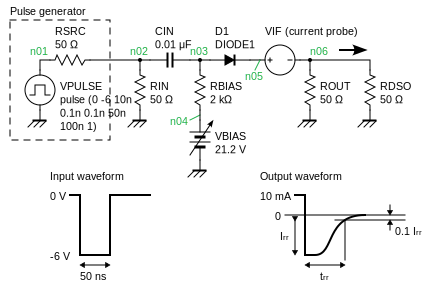
\includegraphics[width=0.8\textwidth]{images/img07.pdf}
    \caption{Test circuit for reverse recovery time}
    \label{fig:img07}
\end{figure}

\begin{lstlisting}[label=listing13,caption=D\_REVERSE\_RECOVERY\_TIME.spice]
D_REVERSE_RECOVERY_TIME.spice
* This script performs a transient analysis to measure the reverse recovery time
* of a diode when switching from forward to reverse bias.

* Diode model
.model DIODE1 D (
.include model.txt
+ )

* Test circuit
VPULSE  n01 0   dc 0 pulse(0 -6 10n 0.1n 0.1n 50n 100n 1) $ Pulse source
RSRC    n01 n02 50      $ Source output resistance (50 Ohm)
RIN     n02 0   50      $ Input resistor
CIN     n02 n03 0.01u   $ DC blocking capacitor
RBIAS   n03 n04 2k      $ Bias resistor to set forward current
VBIAS   n04 0   dc 21.2 $ Bias voltage source for forward conduction
D1      n03 n05 DIODE1  $ Test diode
VIF     n05 n06 dc 0    $ Current probe for diode
ROUT    n06 0   50      $ Output resistor
RDSO    n06 0   50      $ Oscilloscope input resistance (50 Ohm)

.control
* Transient analysis: 10 ps step, 20 ns total time
tran 10p 20n

* Write diode current waveform to file
wrdata D_REVERSE_RECOVERY_TIME.txt i(VIF)

.endc
.end
\end{lstlisting}

Figure \ref{fig:img08} shows a screenshot after tuning the $t_{rr}$ characteristics.
Here, the parameter \texttt{TT} (transit time) is adjusted. According to the datasheet of 1n4148,
the reverse recovery time is specified as $t_{rr}$=3.2 ns under the condition of $I_F$=10 mA and
$I_{rr}$=10 mA. The simulated waveform successfully reproduces this characteristic.

\begin{figure}[htbp]
    \centering
    \includegraphics[width=0.8\textwidth]{images/img08.png}
    \caption{Reverse recovery time}
    \label{fig:img08}
\end{figure}

\end{document}


